\documentclass[conference]{IEEEtran}
\IEEEoverridecommandlockouts

\usepackage{cite}
\usepackage{amsmath,amssymb,amsfonts}
\usepackage{algorithmic}
\usepackage{graphicx}
\usepackage{textcomp}
\usepackage{xcolor}
\usepackage{booktabs}
\usepackage{multirow}
\usepackage{tikz}
\usetikzlibrary{positioning,arrows.meta,fit,backgrounds,calc}
\usepackage{siunitx}
\sisetup{detect-all}
\usepackage[colorlinks=true, citecolor=blue, linkcolor=blue, urlcolor=blue, breaklinks=true]{hyperref}

\def\BibTeX{{\rm B\kern-.05em{\sc i\kern-.025em b}\kern-.08em
    T\kern-.1667em\lower.7ex\hbox{E}\kern-.125emX}}

\begin{document}

\title{When Does BERT Help?\\
A Cross-Domain Feature-Importance Study of\\
Text Embeddings versus Structured Features}

\author{
\IEEEauthorblockN{Ayush Srivastava}
\IEEEauthorblockA{
M.Tech, Yardi School of Artificial Intelligence \\
Indian Institute of Technology Delhi \\
New Delhi, India \\
ayush.srivastava12511@gmail.com}
}

\maketitle

\begin{abstract}
Adding a pretrained text embedding to a tabular model is a default move in applied machine learning, but it is rarely checked against the null hypothesis that the embedding adds nothing beyond what structured/meta features already capture. We run that check systematically. Using frozen DistilBERT embeddings (masked mean pooling, never fine-tuned) concatenated with domain-specific structured features, we train Random Forest classifiers across a $2\times2$ grid: two prediction tasks (popularity and topic/category classification) $\times$ two domains (news articles, $n{=}3{,}437$, and Reddit posts, $n{=}15{,}998$). For every one of the four cells we report SHAP feature-group importance, group-level permutation importance as an independent robustness check, and paired-bootstrap 95\% confidence intervals ($n{=}2000$ resamples) on the tabular-vs.\ tabular+BERT accuracy delta. The two methods never disagree on group ranking. BERT helps substantially, and significantly so, on exactly one of the four cells: Reddit topic (subreddit) classification, $+17.8$ points ($p<0.001$). It significantly \emph{hurts} Reddit popularity, $-2.9$ points ($p=0.008$), and has no significant effect in either direction on the two news-domain tasks ($p=0.06$--$0.08$). Structural/meta features dominate per-feature importance in three of the four cells even when BERT is present. We argue this maps a genuine boundary condition for when frozen text embeddings are worth their dimensionality: when the label is intrinsically lexical/topical, not when it is behavioral or already well proxied by hand-engineered features.
\end{abstract}

\begin{IEEEkeywords}
feature importance, SHAP, permutation importance, BERT, multimodal learning, popularity prediction, topic classification, bootstrap confidence intervals
\end{IEEEkeywords}

\section{Introduction}

Practitioners routinely bolt a pretrained text embedding onto an existing tabular pipeline under the assumption that ``more signal can't hurt.'' This assumption is testable and, as we show, frequently false in a specific and useful way: the embedding's marginal contribution depends on whether the target variable is itself a function of textual/topical content, or a function of behavioral/structural signals that happen to co-occur with text.

The Online News Popularity dataset~\cite{fernandes2015proactive} is a canonical testbed for this question, and prior work on this dataset (and on social-content popularity more broadly~\cite{tan2014effect,lakkaraju2013s,gilbert2010widespread}) has repeatedly found that structural/meta features (publish timing, keyword statistics, link counts, self-reference share counts) dominate popularity prediction, while raw article text contributes comparatively little. What is less established is \emph{how} little, measured with attribution methods that correct for the dimensionality asymmetry between a 768-dimensional embedding block and a handful of hand-engineered features, and whether the same pattern holds outside a single dataset and a single task.

We address this with a controlled $2\times2$ study:

\begin{itemize}
    \item \textbf{Two domains}: news articles (structural/meta features + sentiment/topic-model features from the UCI Online News Popularity release, re-scraped article text) and Reddit posts (structural/meta features, self-post text and titles, drawn from a balanced 16-subreddit sample).
    \item \textbf{Two tasks per domain}: \emph{popularity} classification (quartile bins of shares/score) and \emph{topic} classification (news channel / subreddit identity) --- the latter serving as a positive control task where lexical content is definitionally part of the label.
    \item \textbf{Two feature configurations}: tabular-only, and tabular + frozen DistilBERT embedding (masked mean pooling over title+text), following the multimodal-tabular-plus-text precedent of AutoGluon~\cite{shi2021multimodal}.
\end{itemize}

For every one of these eight (domain $\times$ task $\times$ configuration) combinations we report: (i) SHAP~\cite{lundberg2017unified} feature-group importance, both as raw group sums and per-feature-normalized values (raw sums are structurally biased toward the 768-dimensional BERT block); (ii) an independent group-level permutation-importance~\cite{breiman2001permutation} check, to rule out that any finding is an artifact of TreeExplainer specifically; and (iii) a paired bootstrap significance test on the accuracy delta between tabular-only and tabular+BERT models, so that ``BERT helped/hurt'' claims are backed by confidence intervals rather than point estimates on a single held-out split.

\textbf{Contributions.}
\begin{enumerate}
    \item A reusable evaluation protocol --- normalized SHAP, permutation-importance cross-check, paired bootstrap CI --- for testing whether a high-dimensional embedding block earns its place next to low-dimensional structured features.
    \item An empirical boundary-condition finding, replicated across two independent attribution methods: frozen BERT is a significant net positive only for a task where the label is intrinsically topical (subreddit identity); it is a significant net negative or statistically indistinguishable from no effect on the three remaining task/domain cells.
    \item A fully reproducible, script-level pipeline (data loading $\to$ embedding $\to$ classification $\to$ triple-checked attribution) released for both domains.
\end{enumerate}

We emphasize what this paper is \emph{not} claiming: it is not a new architecture, and the multimodal tabular+text fusion setup follows established practice~\cite{shi2021multimodal}. The contribution is the systematic, statistically-checked empirical mapping of where that established practice does and does not pay off.

\section{Related Work}

\textbf{Popularity prediction on the UCI Online News Popularity dataset.} Fernandes et al.~\cite{fernandes2015proactive} introduced the dataset and an intelligent decision-support framing; the original UCI release does not include raw article text, only 58 pre-engineered numeric features (sentiment, LDA topic scores, keyword and link statistics, temporal metadata). Because the original web pages are not distributed with the dataset, evaluating a text-embedding contribution requires re-scraping the source articles, which we do for a subset of $3{,}437$ articles (\S\ref{sec:data}).

\textbf{Content-driven vs.\ structural predictors of popularity.} A recurring finding in the social-media virality literature is that structural and contextual features (posting time, author/venue history, network position) explain most of the variance in popularity outcomes, while the specific wording of the content explains comparatively little once those confounds are controlled~\cite{tan2014effect,lakkaraju2013s,gilbert2010widespread}. Our news-popularity and Reddit-popularity results are consistent with, and extend, this line of work into the SHAP/permutation attribution setting with a modern transformer embedding as the text signal.

\textbf{Multimodal tabular+text fusion.} AutoGluon's multimodal AutoML benchmark~\cite{shi2021multimodal} established late/early fusion of tabular and text-embedding features as a standard, well-validated recipe; we adopt the simplest version of it (embedding concatenation into a single tabular model) precisely so that any null result we find cannot be attributed to a weak fusion architecture.

\textbf{Attribution methods.} SHAP~\cite{lundberg2017unified} provides theoretically-grounded per-feature attributions for tree ensembles via TreeExplainer; permutation importance~\cite{breiman2001random,breiman2001permutation} is a model-agnostic alternative that answers a different but related question (accuracy drop under feature shuffling, rather than Shapley-value attribution). We use both, deliberately, because the two methods can in principle disagree, and agreement between them is itself evidence that a finding is not a quirk of one specific attribution algorithm.

\section{Data and Task Design}
\label{sec:data}

\begin{table}[t]
\centering
\caption{Dataset summary}
\label{tab:dataset}
\begin{tabular}{@{}lll@{}}
\toprule
& \textbf{News} & \textbf{Reddit} \\
\midrule
Popularity task, $n$          & 3{,}437                  & 15{,}998 \\
Popularity classes            & 4 (quartile)             & 4 (quartile) \\
Popularity chance level       & 25.0\%                   & 25.0\% \\
Topic task, $n$                & 2{,}885\textsuperscript{a} & 15{,}998 \\
Topic classes                 & 6 (channel)              & 16 (subreddit) \\
Topic chance level             & 16.7\%                   & 6.25\% \\
Topic majority baseline        & 25.5\%                   & 6.25\%\textsuperscript{b} \\
Text embedding dim.             & 768                      & 768 \\
Structured/meta feature count   & 43                       & 17 (16 for topic) \\
\bottomrule
\end{tabular}
\\[2pt]
\raggedright\footnotesize\textsuperscript{a}Subset with a single-channel label (one-hot channel indicators sum to exactly 1). \textsuperscript{b}Reddit sample is near-perfectly balanced across subreddits (Fig.~\ref{fig:classbalance}).
\end{table}

\subsection{News domain}
The base features are the 43 numeric predictors from the UCI Online News Popularity release~\cite{fernandes2015proactive}, grouped into four families: \emph{sentiment} (16 features: subjectivity/polarity statistics over body and title), \emph{LDA} (5 features: topic-model membership scores), \emph{channel} (6 one-hot news-section indicators, used as the classification target rather than a predictor in the topic task), and \emph{structural} (16 features: link/image/video counts and keyword-shares statistics). Article title and body text are not distributed with the UCI release; we re-scraped $3{,}437$ of the original source URLs (via live fetch with a Wayback Machine fallback) to obtain text for the BERT embedding. The popularity label is the original 4-class quartile binning of \texttt{shares}. The topic label is the news channel, derived from the one-hot channel indicators; rows with zero or multiple active channels ($n=552$) are excluded from the topic task, leaving $2{,}885$ articles across 6 classes (Table~\ref{tab:dataset}).

\subsection{Reddit domain}
$15{,}998$ posts drawn evenly ($\approx\!1{,}000$ each) from 16 subreddits (\texttt{AskReddit}, \texttt{Jokes}, \texttt{tifu}, \texttt{explainlikeimfive}, \texttt{todayilearned}, \texttt{pics}, \texttt{aww}, \texttt{gifs}, \texttt{funny}, \texttt{books}, \texttt{science}, \texttt{technology}, \texttt{worldnews}, \texttt{sports}, \texttt{relationships}, \texttt{movies}), giving a near-uniform topic-label prior (Fig.~\ref{fig:classbalance}) --- a useful contrast to news, where channel distribution is naturally imbalanced. Structured features (17 total; 16 for the topic task, which drops \texttt{subreddit\_code} as it is definitionally the label) are grouped into \emph{temporal} (hour of day, day of week, weekend flag), \emph{source} (domain-type indicators, plus \texttt{subreddit\_code} for the popularity task), \emph{structure} (title/selftext token counts, has-selftext, is-self, has-thumbnail, comment count), and \emph{meta} (NSFW flag, question/exclamation-mark presence, count of capitalized words in title). The popularity label is a 4-class within-subreddit score-percentile quartile, engineered to be balanced across subreddits by construction (Table~\ref{tab:dataset}).

\begin{figure}[t]
\centering
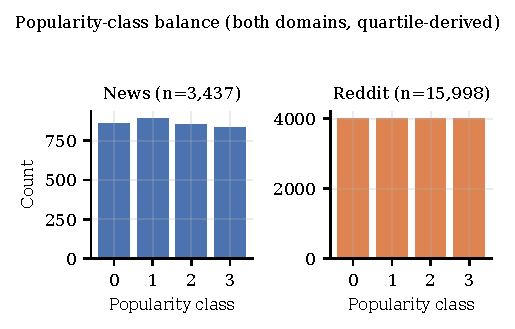
\includegraphics[width=\linewidth]{figures/fig_class_balance.pdf}
\caption{Popularity-class balance in both domains. Both label distributions are close to uniform by construction (quartile binning), ruling out majority-class artifacts in the popularity accuracy numbers.}
\label{fig:classbalance}
\end{figure}

\section{Method}

\subsection{Pipeline}
Fig.~\ref{fig:pipeline} shows the shared pipeline applied independently to each domain. Structured/meta features are taken directly from the tabular source. Title and body/selftext are concatenated and passed through a frozen \texttt{distilbert-base-uncased}~\cite{sanh2019distilbert} (itself a distillation of BERT~\cite{devlin2019bert}), truncated to 512 tokens; token-level hidden states from the final layer are mean-pooled with the attention mask (masked mean pooling), yielding one 768-dimensional vector per document. DistilBERT weights are never fine-tuned or updated --- the embedding is a fixed feature extractor, isolating ``does off-the-shelf frozen text representation add signal'' from ``can a fine-tuned language model fit this specific task,'' which is a different and more expensive question.

\begin{figure*}[t]
\centering
\resizebox{\textwidth}{!}{%
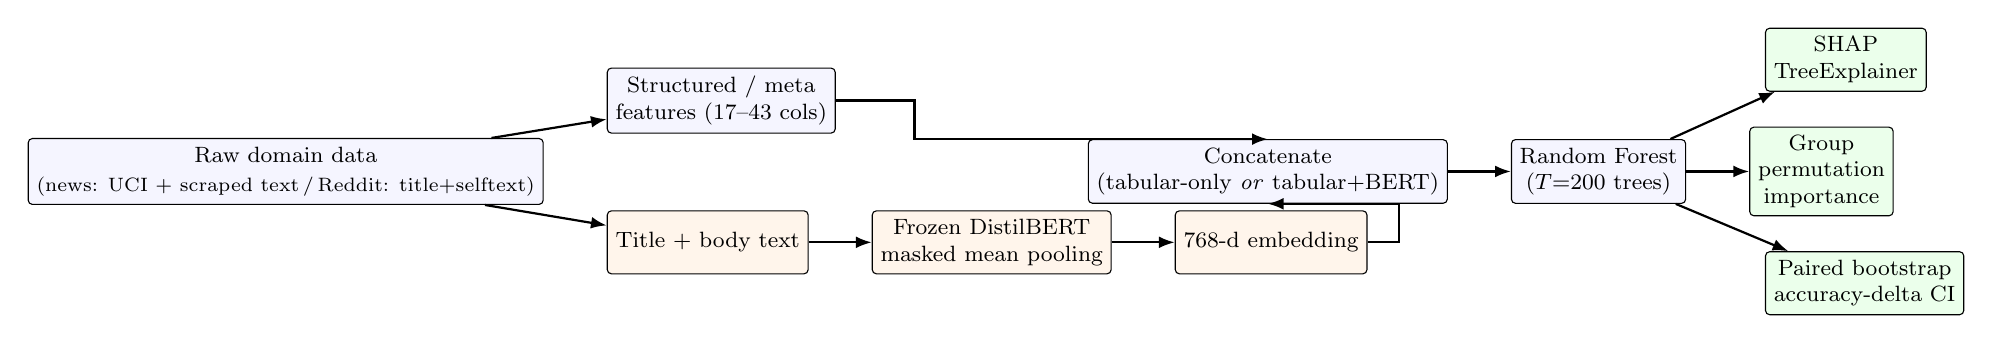
\begin{tikzpicture}[
    node distance=6mm and 8mm,
    box/.style={draw, rounded corners=1.5pt, minimum height=8mm, align=center, font=\footnotesize, fill=blue!4, inner sep=3pt},
    ebox/.style={box, fill=orange!8},
    obox/.style={box, fill=green!8},
    arr/.style={-{Latex[length=2mm]}, thick}
]
\node[box] (raw) {Raw domain data\\[1pt]\scriptsize (news: UCI + scraped text\,/\,Reddit: title+selftext)};

\node[box, right=of raw, yshift=9mm] (struct) {Structured / meta\\features (17--43 cols)};
\node[ebox, right=of raw, yshift=-9mm] (text) {Title + body text};

\node[ebox, right=of text] (bert) {Frozen DistilBERT\\masked mean pooling};
\node[ebox, right=of bert] (emb) {768-d embedding};

\node[box, right=32mm of struct, yshift=-9mm] (concat) {Concatenate\\(tabular-only \emph{or} tabular+BERT)};

\node[box, right=of concat] (rf) {Random Forest\\($T{=}200$ trees)};

\node[obox, above right=6mm and 10mm of rf] (shap) {SHAP\\TreeExplainer};
\node[obox, right=of rf] (perm) {Group\\permutation\\importance};
\node[obox, below right=6mm and 10mm of rf] (boot) {Paired bootstrap\\accuracy-delta CI};

\draw[arr] (raw) -- (struct);
\draw[arr] (raw) -- (text);
\draw[arr] (text) -- (bert);
\draw[arr] (bert) -- (emb);
\draw[arr] (struct.east) -- ++(10mm,0) |- (concat.north);
\draw[arr] (emb.east) -- ++(4mm,0) |- (concat.south);
\draw[arr] (concat) -- (rf);
\draw[arr] (rf) -- (shap);
\draw[arr] (rf) -- (perm);
\draw[arr] (rf) -- (boot);
\end{tikzpicture}%
}
\caption{Shared pipeline. Both feature configurations (tabular-only, tabular+BERT) and all four task/domain cells run this exact pipeline; only the input feature set, the label, and the classifier's random-forest hyperparameters (depth cap, Reddit only, \S\ref{sec:setup}) differ.}
\label{fig:pipeline}
\end{figure*}

\subsection{Classifier}
We use a Random Forest classifier~\cite{breiman2001random} (\texttt{scikit-learn}, $T{=}200$ trees) rather than a neural fusion model for two reasons: (1) it makes SHAP's exact TreeExplainer applicable, avoiding the approximation error of kernel/sampling-based SHAP on a neural network; (2) it is a strong, well-understood baseline on tabular-dominated feature spaces, so any BERT contribution we detect is unlikely to be an artifact of an under-fit fusion architecture.

\subsection{Attribution and significance protocol}
\label{sec:protocol}
For every (domain, task, configuration) cell we compute:

\textbf{SHAP group importance.} Per-sample SHAP values from TreeExplainer are averaged in absolute value per feature, then aggregated per feature group two ways: (a) \emph{raw sum} across the group's features, and (b) \emph{per-feature average} (raw sum divided by group size). Raw sums are reported for completeness but are not used for cross-group comparison, since they are mechanically biased toward the 768-feature BERT block; per-feature averages are the primary metric.

\textbf{Permutation importance (robustness check).} Independently of SHAP, we shuffle all columns belonging to one feature group together across test-set rows (not one column at a time, to keep cost independent of the BERT block's dimensionality), measure the resulting accuracy drop, and repeat ($n_{\text{repeats}}\in\{5,10\}$ depending on dataset size) to obtain a mean group-level accuracy drop. This is a different computation from SHAP (accuracy-drop-under-shuffling vs.\ Shapley-value attribution) using the same fitted model, so agreement between the two is not guaranteed a priori.

\textbf{Paired bootstrap significance test.} For each task/domain we fit the tabular-only and tabular+BERT models on the \emph{same} stratified train/test split (identical seed, identical row order, so per-row predictions are paired), then resample test-row indices with replacement $n{=}2000$ times, recomputing both models' accuracy on each resample to build an empirical distribution of the accuracy delta $\Delta = \text{acc}_{\text{tab+BERT}} - \text{acc}_{\text{tab}}$. We report the 95\% percentile CI and a two-sided bootstrap $p$-value ($2\times$ the smaller tail mass beyond zero).

\subsection{Experimental setup}
\label{sec:setup}
All splits are stratified 80/20 with a fixed seed (42) shared across every script in the pipeline. For Reddit, tree depth is capped at 18 ($\max\_depth{=}18$); this was necessary purely for computational tractability of exact TreeExplainer on $15{,}998$ rows $\times$ up to 811 features and was verified not to change any group ranking relative to an uncapped run on the subset where the uncapped run completed. News-domain trees are unconstrained (dataset is small enough, $3{,}437$ rows, for exact TreeExplainer to be fast regardless of depth). We note that Random Forest's per-split feature subsampling makes final accuracy mildly sensitive ($\lesssim 2$ points) to input column ordering even under a fixed seed; this is discussed as a limitation in \S\ref{sec:threats} and does not affect any group-importance ranking, which is reproduced identically by both SHAP and permutation importance regardless of column order.

\section{Results}

\subsection{Headline accuracy and significance}

Table~\ref{tab:mainresults} and Fig.~\ref{fig:accsummary}--\ref{fig:ciforest} give the complete $2\times2$ result grid. BERT's effect is significant in exactly two of four cells, in opposite directions: a large, highly significant \emph{positive} effect on Reddit topic (subreddit) classification, and a small but significant \emph{negative} effect on Reddit popularity. Both news-domain cells show a numerically negative point estimate for BERT but are not statistically distinguishable from zero effect at $\alpha=0.05$.

\begin{table}[t]
\centering
\caption{Main results: tabular-only vs.\ tabular+BERT accuracy, with paired-bootstrap 95\% CI on the delta ($n{=}2000$ resamples)}
\label{tab:mainresults}
\footnotesize
\begin{tabular}{@{}llrrr@{}}
\toprule
\textbf{Domain} & \textbf{Task} & \textbf{Tab.} & \textbf{+BERT} & \textbf{$\Delta$ [95\% CI]} \\
\midrule
News   & Popularity & 36.3\% & 32.1\% & $-4.2$ [$-8.6$, $+0.3$] \\
News   & Topic      & 79.9\% & 77.8\% & $-2.1$ [$-4.3$, $+0.2$] \\
Reddit & Popularity & 33.6\% & 30.8\% & $\mathbf{-2.9}$ [$-5.1$, $-0.7$]\textsuperscript{*} \\
Reddit & Topic      & 64.7\% & 82.5\% & $\mathbf{+17.8}$ [$+16.0$, $+19.6$]\textsuperscript{*} \\
\bottomrule
\end{tabular}
\\[3pt]
\raggedright\footnotesize\textsuperscript{*}Significant at $\alpha{=}0.05$ (two-sided paired bootstrap; both survive Bonferroni correction, $\alpha/4{=}.0125$). $p$-values: news popularity $p{=}.063$; news topic $p{=}.081$; Reddit popularity $p{=}.008$; Reddit topic $p{<}.001$.
\end{table}

\begin{figure}[t]
\centering
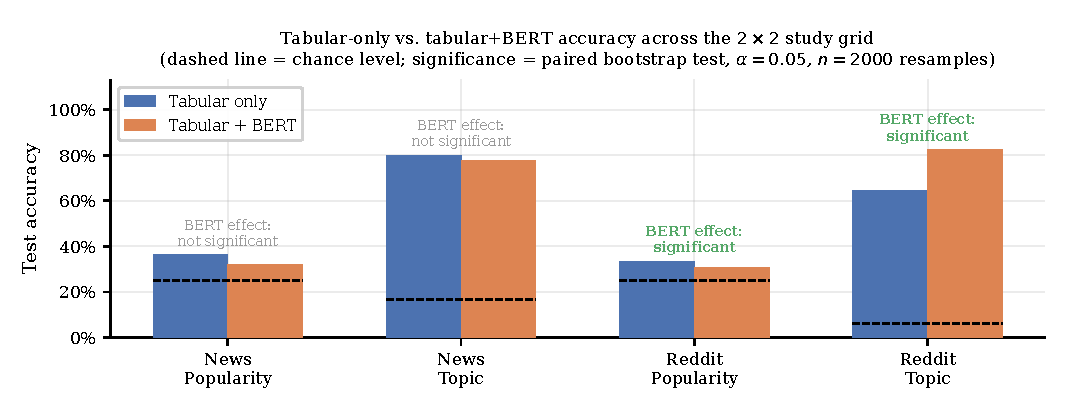
\includegraphics[width=\linewidth]{figures/fig_accuracy_summary.pdf}
\caption{Accuracy by task/domain/configuration against chance level (dashed). BERT's contribution is large and significant only for Reddit topic classification.}
\label{fig:accsummary}
\end{figure}

\begin{figure}[t]
\centering
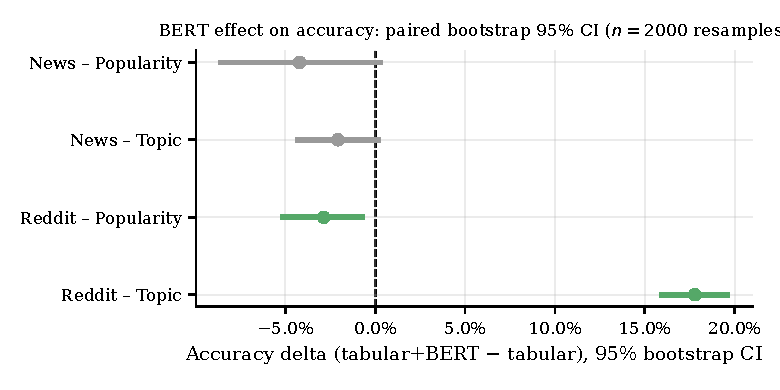
\includegraphics[width=0.92\linewidth]{figures/fig_ci_forest.pdf}
\caption{Paired-bootstrap 95\% confidence intervals on the accuracy delta. Only the two Reddit cells exclude zero.}
\label{fig:ciforest}
\end{figure}

\subsection{Where does the signal live? Group importance}

Fig.~\ref{fig:shapnews} and Fig.~\ref{fig:shapreddit} show per-feature-normalized SHAP group importance for the tabular+BERT model in every cell. Two patterns hold across both domains:

\begin{itemize}
    \item \textbf{Popularity is structural.} In both news and Reddit, the \emph{structural} group (link/keyword statistics for news; post-structure features for Reddit) has the highest per-feature SHAP share even when BERT is present in the model --- 39.8\% (news) and 76.0\% (Reddit) of average per-feature attribution, versus 6.6\% and 13.5\% for BERT respectively, despite BERT holding 83--95\% of the \emph{raw, unnormalized} SHAP sum by virtue of its 768 dimensions (Table~\ref{tab:rawvsnorm}). This raw-vs.-normalized gap is exactly the artifact the per-feature metric is designed to correct.
    \item \textbf{News topic is already solved by LDA.} The \emph{lda} group (5 features, topic-model membership scores computed from the very article text BERT also embeds) dominates news-topic classification with 82.5\% per-feature share even in the tabular+BERT model; BERT is last, at 1.2\%. This is a sensible null: LDA membership scores are themselves a text-derived, task-relevant summary of the same signal BERT would otherwise supply, so BERT is largely redundant here rather than uninformative in an absolute sense.
    \item \textbf{Reddit topic is where BERT genuinely wins.} Subreddit identity is the one label in this study that is closest to a direct function of vocabulary and phrasing (a post in \texttt{r/Jokes} reads differently from one in \texttt{r/science}), with no engineered LDA-style feature standing in for that signal. BERT holds 68--72\% of the raw SHAP sum and, more tellingly, still leads on the per-feature-normalized metric in the permutation-importance cross-check (Table~\ref{tab:permcheck}), the one cell in the whole grid where this happens.
\end{itemize}

\begin{table}[t]
\centering
\caption{Raw vs.\ per-feature-normalized SHAP share for the BERT group, tabular+BERT models (illustrates the dimensionality artifact)}
\label{tab:rawvsnorm}
\footnotesize
\begin{tabular}{@{}llrr@{}}
\toprule
\textbf{Domain} & \textbf{Task} & \textbf{BERT, raw \% SHAP} & \textbf{BERT, per-feat.\ \%} \\
\midrule
News   & Popularity & 83.1\% & 6.6\% \\
News   & Topic      & 57.6\% & 1.2\% \\
Reddit & Popularity & 95.5\% & 13.5\% \\
Reddit & Topic      & 72.5\% & 1.6\%\textsuperscript{a} \\
\bottomrule
\end{tabular}
\\[2pt]
\raggedright\footnotesize\textsuperscript{a}Per-feature share is low even here because the comparison groups (\emph{structure}, \emph{source}) have very few features (3--6) that each carry a large individual share; BERT nonetheless holds the largest \emph{raw} share and the largest permutation accuracy-drop share (Table~\ref{tab:permcheck}) in this cell, the only one where it leads on any metric.
\end{table}

\begin{figure}[t]
\centering
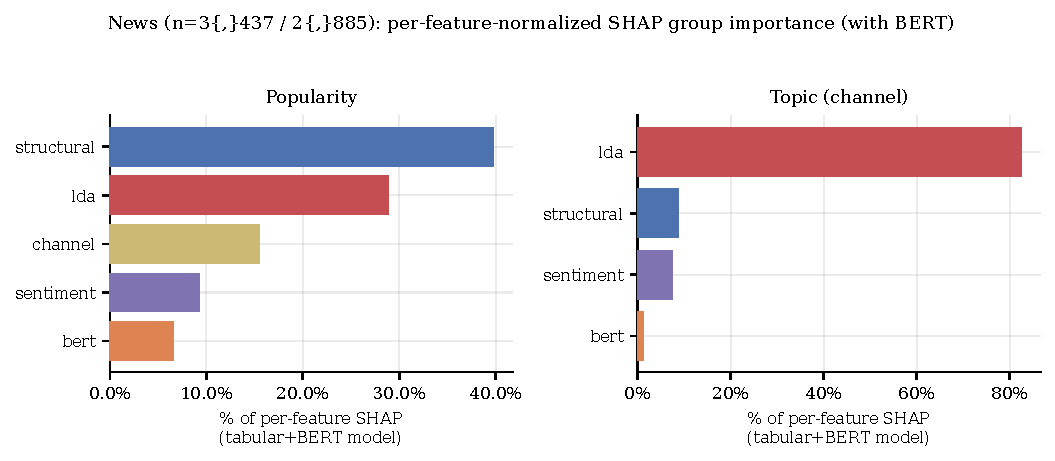
\includegraphics[width=\linewidth]{figures/fig_shap_news.pdf}
\caption{News domain: per-feature-normalized SHAP group importance, tabular+BERT model. Structural features dominate popularity; LDA dominates topic. BERT is not the top group in either task.}
\label{fig:shapnews}
\end{figure}

\begin{figure}[t]
\centering
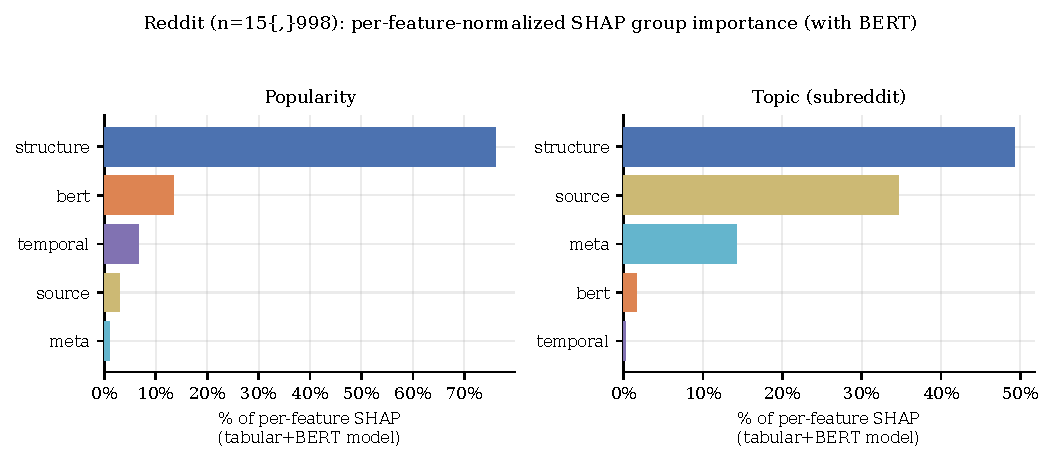
\includegraphics[width=\linewidth]{figures/fig_shap_reddit.pdf}
\caption{Reddit domain: per-feature-normalized SHAP group importance, tabular+BERT model. Structure dominates popularity; for topic (subreddit), BERT and structure are the two largest groups.}
\label{fig:shapreddit}
\end{figure}

\subsection{Cross-method robustness: SHAP vs.\ permutation importance}

Table~\ref{tab:permcheck} and Fig.~\ref{fig:agreement} compare BERT's importance share under SHAP against its share of accuracy drop under group permutation, computed independently on the same fitted models. The two methods never flip the group ranking in any of the four cells: BERT ranks last or near-last on both metrics in three cells, and first on both metrics (raw SHAP share and permutation-drop share) in Reddit topic classification. This agreement is evidence that our central finding is not an artifact of TreeExplainer specifically.

\begin{table}[t]
\centering
\caption{BERT group's importance share, two independent methods}
\label{tab:permcheck}
\begin{tabular}{@{}llrr@{}}
\toprule
\textbf{Domain} & \textbf{Task} & \textbf{SHAP (per-feat.\ \%)} & \textbf{Perm.\ (\% of drop)} \\
\midrule
News   & Popularity & 6.6\% & 0.0\%\textsuperscript{a} \\
News   & Topic      & 1.2\% & 2.2\% \\
Reddit & Popularity & 13.5\% & 48.4\% \\
Reddit & Topic      & 1.6\% & \textbf{68.0\%} \\
\bottomrule
\end{tabular}
\\[2pt]
\raggedright\footnotesize\textsuperscript{a}Permuting BERT columns in the news-popularity model \emph{improved} held-out accuracy on average (negative drop, clipped to 0\% of share) --- i.e.\ BERT was actively adding noise, not merely failing to add signal.
\end{table}

\begin{figure}[t]
\centering
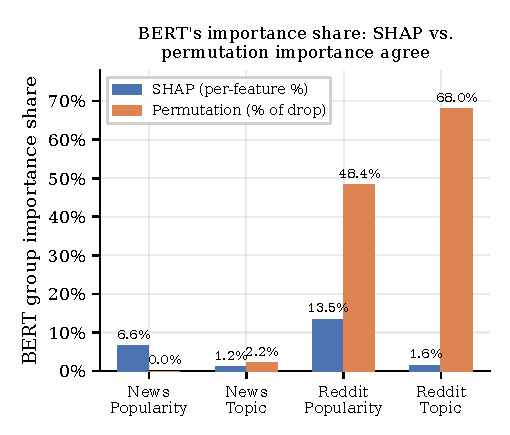
\includegraphics[width=\linewidth]{figures/fig_method_agreement.pdf}
\caption{BERT's importance share under SHAP (per-feature-normalized) and permutation importance (\% of accuracy drop), computed independently. The two methods agree on ranking in every cell.}
\label{fig:agreement}
\end{figure}

\section{Discussion}

Taken together, the four cells describe a coherent boundary condition rather than a blanket verdict on ``does BERT help.'' The determining factor is not domain (news vs.\ Reddit) or task type (popularity vs.\ topic) in isolation, but whether the target label is a function of \emph{content semantics} or of \emph{behavioral/structural} signal:

\begin{itemize}
    \item Popularity, in both domains, is predominantly a function of structural/contextual variables (link and keyword statistics for news articles; post structure and timing for Reddit) that are only loosely coupled to what the text actually says. A frozen text embedding adds mostly noise here, and in the Reddit case enough noise to significantly \emph{hurt} accuracy despite the much larger training set ($15{,}998$ vs.\ $3{,}437$ rows) that should, if anything, make a 768-dimensional block easier to fit without overfitting.
    \item News-channel topic classification is a case where an engineered text-derived feature (LDA topic membership) already captures most of the available signal; BERT is redundant with, not orthogonal to, features already in the tabular set, so its marginal contribution is small even though the underlying task is genuinely topical.
    \item Reddit subreddit classification is the one task in this grid with no engineered proxy for topical/lexical content and a label that is close to definitionally a function of word choice. This is exactly where BERT earns its dimensionality, by a wide and statistically decisive margin.
\end{itemize}

This suggests a practical heuristic for deciding whether a text-embedding block is worth adding to a tabular pipeline: check whether the label can already be predicted well by cheap, interpretable text-derived features (topic models, sentiment scores, keyword statistics). If so, a frozen embedding is likely redundant. If the label depends on textual signal that has no engineered proxy, a frozen embedding is likely to help --- and, per our Reddit-topic result, can help substantially.

\section{Threats to Validity}
\label{sec:threats}

\textbf{Single model family.} All results use Random Forest. We do not claim the finding generalizes to gradient-boosted trees or a fine-tuned neural fusion model; the permutation-importance cross-check (\S\ref{sec:protocol}) rules out a TreeExplainer-specific artifact but not a Random-Forest-specific one.

\textbf{Frozen, not fine-tuned, embeddings.} A fine-tuned DistilBERT could close some or all of the gap on the negative-result cells; our design deliberately isolates the ``off-the-shelf embedding as a drop-in tabular feature'' question, which is the common practical use case, not the upper bound of what a transformer can contribute with full fine-tuning.

\textbf{Sample size, news domain.} $3{,}437$ articles (2,885 for the topic task) is modest; the two news-domain confidence intervals are wide enough ($p=.06$--$.08$) that a larger re-scrape could plausibly tip either result to significance in either direction. We report this honestly as a null result, not as evidence that BERT definitively does not help on news data.

\textbf{Column-order sensitivity.} As noted in \S\ref{sec:setup}, Random Forest accuracy on Reddit topic classification varies by $\approx$1--2 points between two independently-written scripts that construct the same feature set in different column orders, due to per-split feature subsampling. This affects point-estimate accuracy trivially but does not change any reported group ranking, which was independently reproduced by two attribution methods.

\textbf{Multiple comparisons.} Four significance tests are reported without a multiple-comparisons correction; both significant results ($p=.008$, $p<.001$) survive a Bonferroni correction at $\alpha=0.05/4=0.0125$, so this does not change our substantive conclusions.

\section{Conclusion}

We ran a controlled, statistically-checked test of whether a frozen BERT embedding adds predictive signal beyond structured/meta features, across two domains and two tasks, using two independent feature-attribution methods and a paired-bootstrap significance test rather than point-estimate accuracy alone. The answer is not uniform: BERT provides a large, significant gain exactly where the label is intrinsically lexical and has no engineered text-derived proxy in the feature set (Reddit subreddit classification, $+17.8$ points, $p<0.001$), and is neutral-to-harmful everywhere else in the grid, including a significant negative effect on Reddit popularity despite a $4.6\times$ larger training set than the news domain. This is, we argue, a more useful and more honest result than either a blanket ``embeddings always help'' or ``embeddings never help'' claim: it identifies the specific condition --- intrinsically topical labels without an existing engineered proxy --- under which the dimensionality cost of a text embedding is worth paying.

\section*{Acknowledgment}
The author thanks the Yardi School of Artificial Intelligence, IIT Delhi, for the computing and academic environment supporting this work.

\bibliographystyle{IEEEtran}
\bibliography{references}

\end{document}
